\documentclass[12pt]{article}

\usepackage[utf8]{inputenc}
\usepackage[bulgarian]{babel}
\usepackage{graphicx}
\usepackage{sidecap}
\usepackage{amssymb}
\usepackage{amsmath}
\usepackage{hyperref}
\usepackage{commath}
\usepackage{float}
\usepackage[top=1.3in, bottom=1.5in, left=1.3in, right=1.3in]{geometry}


\begin{document}
\begin{center}
\LARGE{\textbf{Тема: Уеб приложение за водене на дневник с възможност за записване и управление на бележки, реализирано с използване на облачните услуги AWS S3, Amazon Cognito, AWS API Gateway, AWS Lambda и Amazon DynamoDB}}

\bigskip
\Large{Предмет: Приложно-програмни интерфейси за работа с облачни архитектури с Амазон Уеб Услуги (AWS)}

\medskip
\Large{Изготвил: Йоанна Миленова Ненкова, фн: 7MI0800263, имейл: anni.nenkova@gmail.com}

\medskip
\Large{Лектор: проф. д-р Милен Петров, година: 2025}

\bigskip
\end{center}

\newpage
\tableofcontents
\bigskip
\bigskip
\newpage

\section{Условие}

\noindent Разработка на уеб приложение, базирано на облачната платформа Amazon Web Services (AWS), което предствлява дигитален дневник. Системата трябва да позволява на потребителя да се регистрира, да създава, редактира и трие дневникови записи, както и да преглежда стари такива.

\medskip

\noindent Потребителят преминава през следните основни стъпки:
\begin{enumerate}
\item Регистрация и потвърждение на акаунт чрез имейл.
\item Вход в системата с валидни идентификационни данни.
\item Създаване на нов запис в дневника със заглавие и съдържание.
\item Преглед на списък с предишни записи.
\item Редактиране или изтриване на съществуващи записи.
\end{enumerate}

\section{Въведение}

В ерата на облачните технологии и сървърлес архитектурите, изграждането на уеб приложения става все по-гъвкаво, бързо и икономически изгодно. Настоящият проект представлява уеб базиран дневник, изграден върху AWS, който позволява на потребителите да записват важни събития и мисли, достъпни от всяко устройство с интернет връзка.

\\
\\
\noindent Основните функционалности включват:
\begin{itemize}
\item Сигурна регистрация и автентикация на потребители чрез Amazon Cognito.
\item Създаване, редактиране и изтриване на дневникови записи.
\item Съхранение на данните в Amazon DynamoDB.
\item API слой за управление на данните, реализиран чрез AWS API Gateway и AWS Lambda.
\item Хостване на клиентската част в Amazon S3.
\item Защита на API методите с потребителска автентикация и контрол на достъпа.
\end{itemize}
\\
\noindent Проектът е изграден изцяло върху сървърлес (serverless) технологии на AWS, което гарантира висока мащабируемост, надеждност и оптимизация на разходите, тъй като се плаща само за реално използваното изчислително време, без да се налага поддръжка на сървъри.

\begin{figure}[H]
\centering
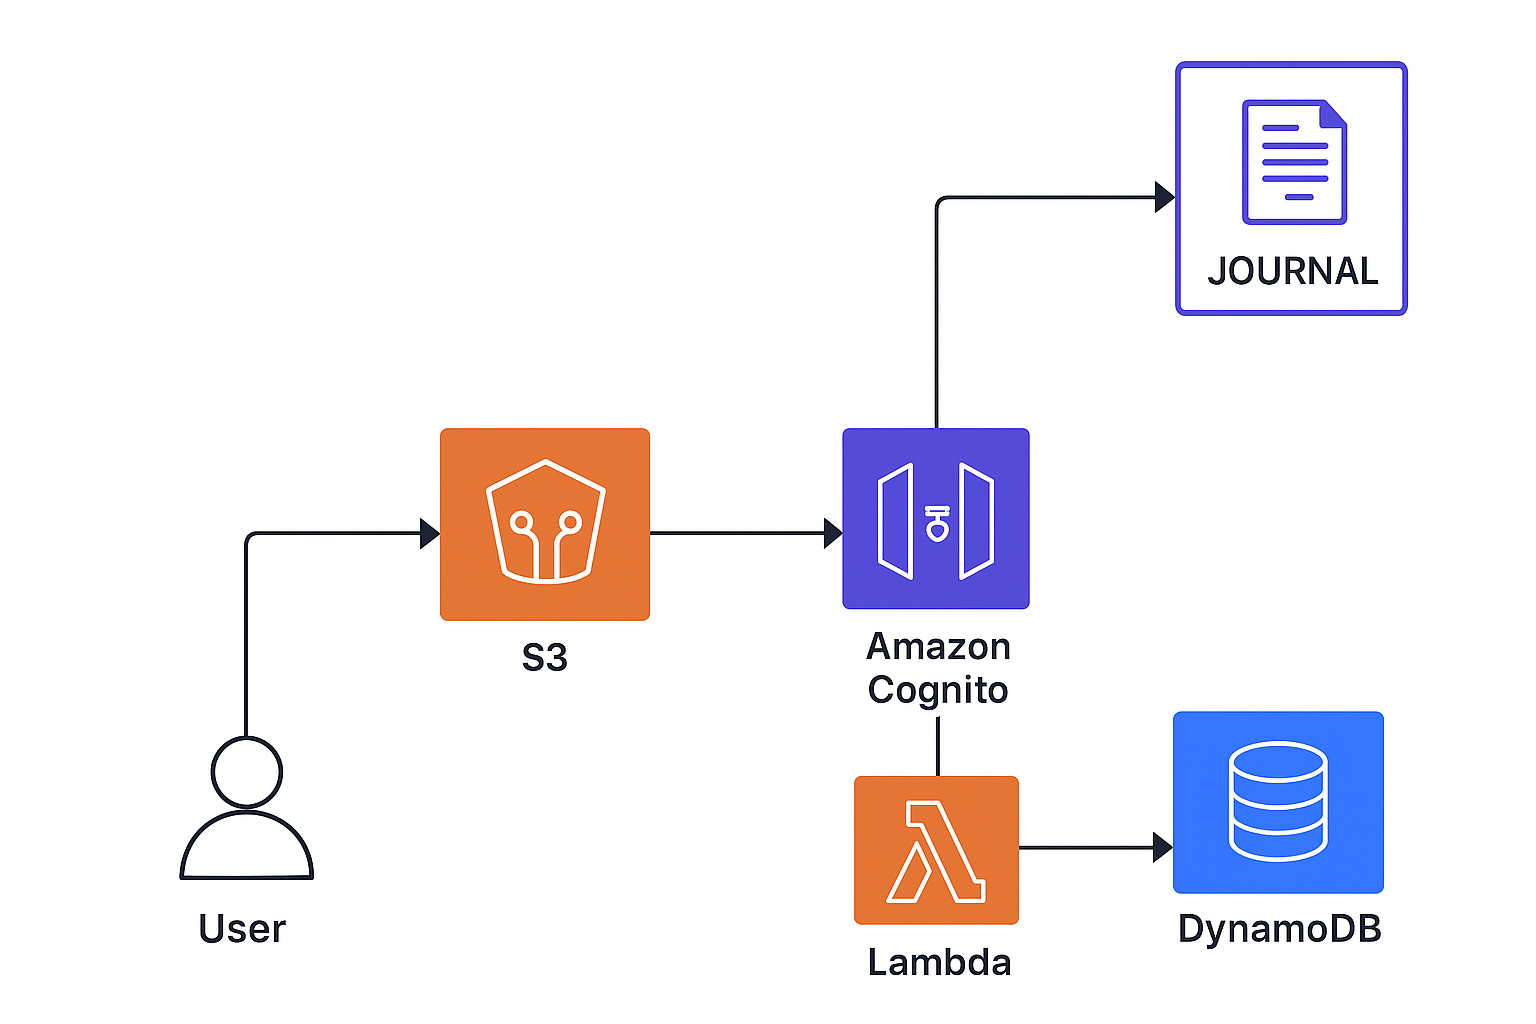
\includegraphics[width=0.9\textwidth]{architecture.png}
\caption{Архитектура на приложението в AWS}
\end{figure}


\section{Теория}
\noindent Архитектурата на проекта се базира на ключови сървърлес услуги от AWS, които позволяват изграждането на модерни, скалируеми и ефективни приложения без необходимост от управление на сървърна инфраструктура.

\subsection{Amazon S3 (Simple Storage Service)}
\textbf{Amazon S3} е услуга за обектно съхранение, която се използва за хостинг на статичните файлове на нашето React уеб приложение (HTML, CSS, JavaScript, изображения). Конфигуриран като уебсайт, S3 bucket служи като начална точка за потребителите, доставяйки бързо и надеждно фронтенд частта на приложението.

\subsection{Amazon Cognito}
\textbf{Amazon Cognito} предоставя цялостно решение за управление на потребителски идентичности. Чрез него се реализира сигурната регистрация, вход и управление на потребителски сесии. Cognito се интегрира директно с API Gateway, за да защитава достъпа до бекенд ресурсите, като гарантира, че само автентикирани потребители могат да извършват определени операции.

\subsection{API Gateway}
\textbf{API Gateway} действа като "входна врата" за всички заявки от клиентското приложение към бекенда. Услугата управлява създаването, публикуването и защитата на RESTful API. Тя приема HTTP заявките, валидира ги (често в комбинация с Cognito), и ги пренасочва (routing) към съответната AWS Lambda функция за обработка.

\subsection{AWS Lambda}
\textbf{AWS Lambda} е сърцето на сървърлес архитектурата. Това е изчислителна услуга, която изпълнява код (в нашия случай Node.js) в отговор на събития, каквито са API заявките от API Gateway. Вместо постоянно работещи сървъри, Lambda функциите се стартират само при нужда, обработват заявката и спират, което води до изключителна ефективност на разходите.

\subsection{Amazon DynamoDB}
\textbf{Amazon DynamoDB} е бърза и гъвкава NoSQL база данни, идеална за сървърлес приложения. Нейната схема "on-read" позволява съхранението на разнородни данни без фиксирана структура. В проекта се използва за съхранение на информация за записи в дневник. Гарантира ниска латентност и автоматично мащабиране.


%\newpage

\section{Използвани технологии}
\begin{itemize}
\item \textbf{Amazon S3 (Simple Storage Service)} - Обектно хранилище, използвано за хостинг на статичните файлове на React приложението (CSS, JavaScript).\\

\item \textbf{Amazon Cognito} - Услуга за управление на потребителски идентичности и автентикация. Осигурява сигурна регистрация и вход в системата.\\

\item \textbf{Amazon API Gateway} - Управлявана услуга за създаване, публикуване и защита на RESTful APIs. Служи като входна точка за всички заявки от фронтенда към бекенда.\\

\item \textbf{AWS Lambda} - Serverless compute услуга, която изпълнява бекенд логиката (Node.js 18.x), без да е необходимо да се управляват сървъри.\\

\item \textbf{Amazon DynamoDB} - Бърза и гъвкава NoSQL база данни за съхранение на информация за потребители и техните записи в дневник.\\
\end{itemize}

%\newpage

\section{Инсталация и настройки}

\noindent\textbf{Стъпка 1.} Конфигуриране на DynamoDB таблица за съхранение на данните. Използваме DynamoDB, защото предлага автоматично мащабиране, ниска латентност и лесна интеграция със сървърлес приложения. За разлика от релационни бази като RDS, които изискват управление на сървъри и фиксирани схеми, или документоориентирани бази като MongoDB, които изискват сами да настроите кластер и резервни копия, DynamoDB е напълно управлявана и гарантира надеждност и висока производителност дори при голямо натоварване.
\\
\\
\noindent\textbf{1.1.} Създаване на таблицата.\\
Table name: JournalEntries,\\
Partition key: userId (Тип: String) - тук ще пазим уникалния идентификатор на потребителя от Cognito,\\
Sort key: entryId (Тип: String) - това ще бъде уникален ID за всеки запис в дневника.

 \begin{figure}[H]
\centering
    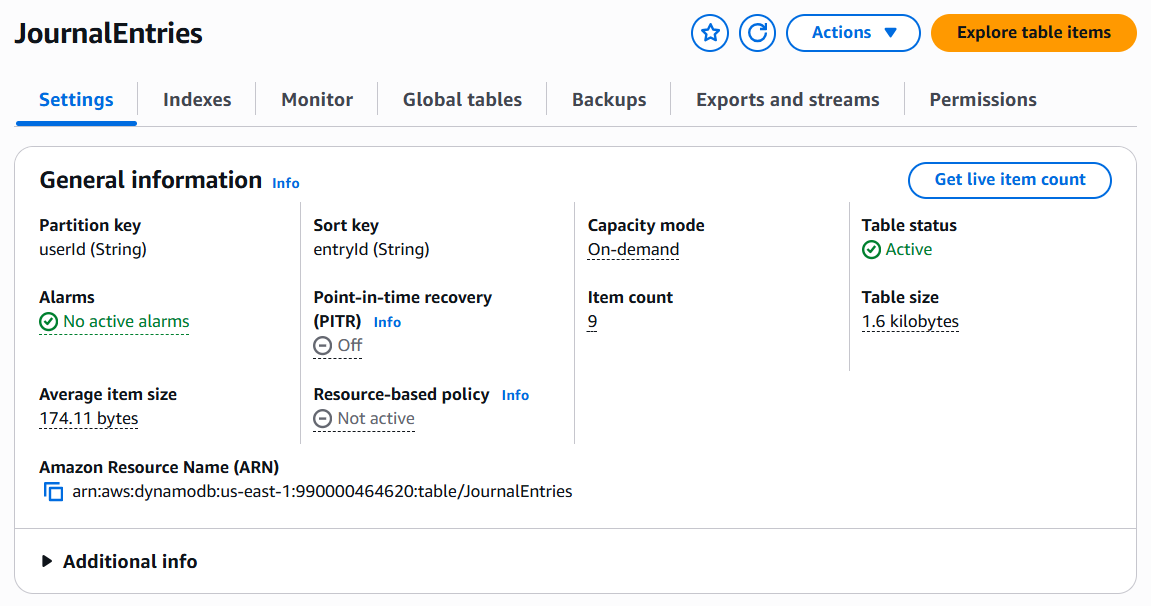
\includegraphics[scale=0.4]{table.png}
  \caption{JournalEntries Table в AWS Management Console}
\end{figure}

\noindent\textbf{1.2.} Създаване на Global Secondary Index за извличане на записи по дата.\\
GSI name: userId-createdAt-index,\\
Partition key: userId (Тип: String),\\
Sort key: createdAt (Тип: String) - тук ще пазим дата и час на създаване на записа.

 \begin{figure}[H]
\centering
    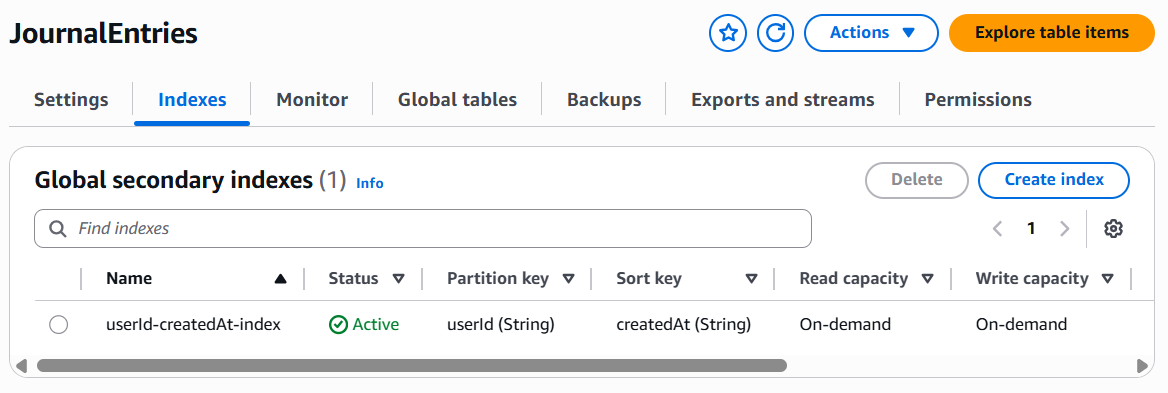
\includegraphics[scale=0.4]{gsi.png}
  \caption{JournalEntries Indexes в AWS Management Console}
\end{figure}

\medskip

\noindent\textbf{Стъпка 2.} Конфигуриране на Cognito User pool и App client за автентикация на потребителите.\\
\noindent\textbf{2.1.} Създаване на Cognito User pool-а. Изисква имейл за регистрация.\\
User pool name: User pool - -vutgn,\\
Region: us-east-1,\\
User pool ID: us-east-1$_$DeXYhj08z.\\

 \begin{figure}[H]
\centering
    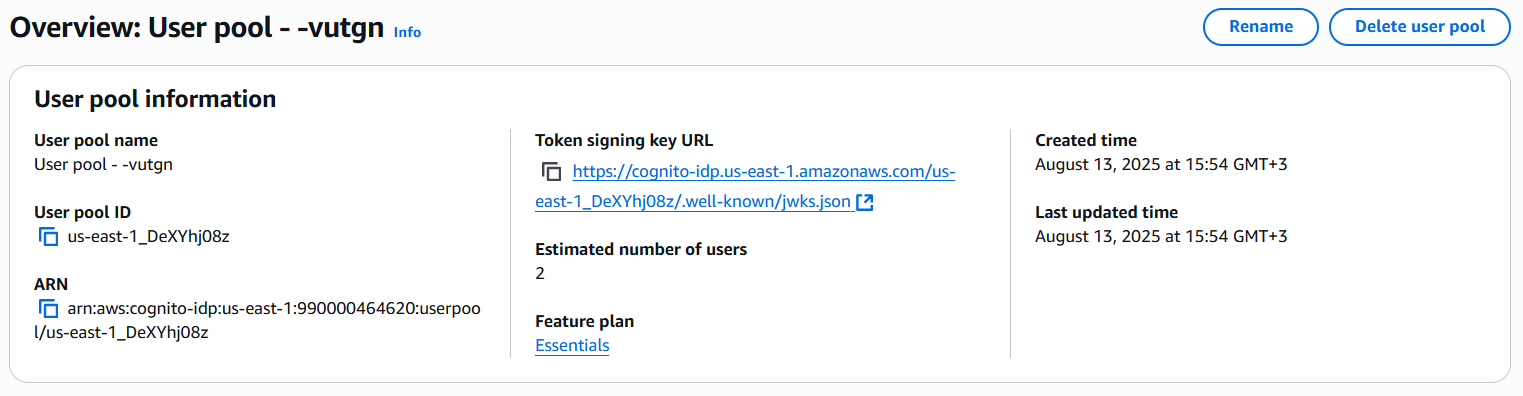
\includegraphics[scale=0.4]{user_pool.png}
  \caption{User pool в AWS Management Console}
\end{figure}

\noindent\textbf{2.2.} Създаване на App client. Представлява Single Page Application.\\
Client name: Journal,\\
Client ID: 53n4r1l0qci7hkvdkh84penpkg.\\

 \begin{figure}[H]
\centering
    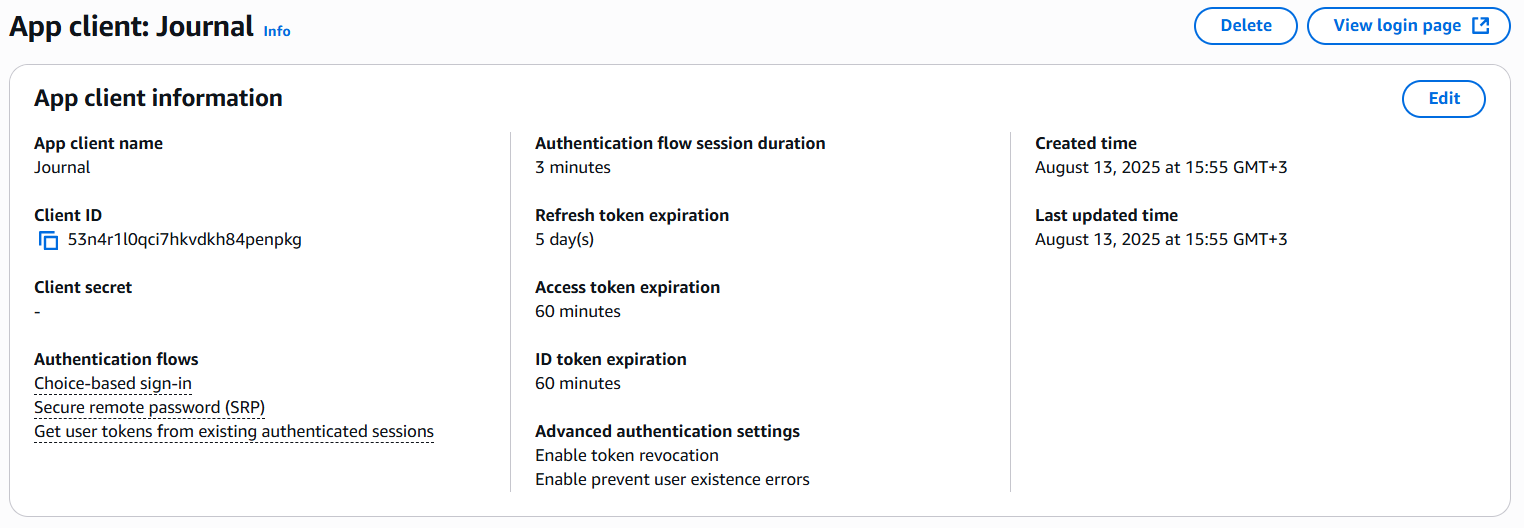
\includegraphics[scale=0.4]{app_client.png}
  \caption{App client в AWS Management Console}
\end{figure}

\medskip

\noindent\textbf{Стъпка 3.} Създаване на Lambda функции за управление на записите.
Всяка Lambda функция е микросервиз, който отговаря за конкретна операция с данните в DynamoDB. Функциите обработват HTTP заявки от API Gateway, взаимодействат с базата данни и връщат резултат. Те включват логика за валидация на входящите данни, обработка на грешки (например, записът не е намерен или потребителят няма права за достъп) и форматиране на отговора, за да бъдат коректно обработени от фронтенда.
\\
\\
\noindent\textbf{3.1.} Функция \texttt{getEntries} за извличане на записи по дата на създаване. Тя прави заявка към DynamoDB, използвайки Global Secondary Index (\texttt{userId-createdAt-index}), за да върне всички записи на конкретен потребител, сортирани по дата на създаване.\\
\noindent\textbf{3.2.} Функция \texttt{createEntry} за създаване на запис. Тя получава данни (заглавие, съдържание) от заявката, генерира уникален ID за записа и го съхранява в DynamoDB.\\
\noindent\textbf{3.3.} Функция \texttt{editEntry} за редактиране на запис. Тя приема ID на запис и нови данни, след което обновява съществуващия запис в DynamoDB, като проверява дали потребителят е собственик на записа.\\
\noindent\textbf{3.4.} Функция \texttt{deleteEntry} за изтриване на запис. Тя премахва запис от DynamoDB въз основа на подаден ID, отново след проверка за правата на достъп на потребителя.\\

 \begin{figure}[H]
\centering
    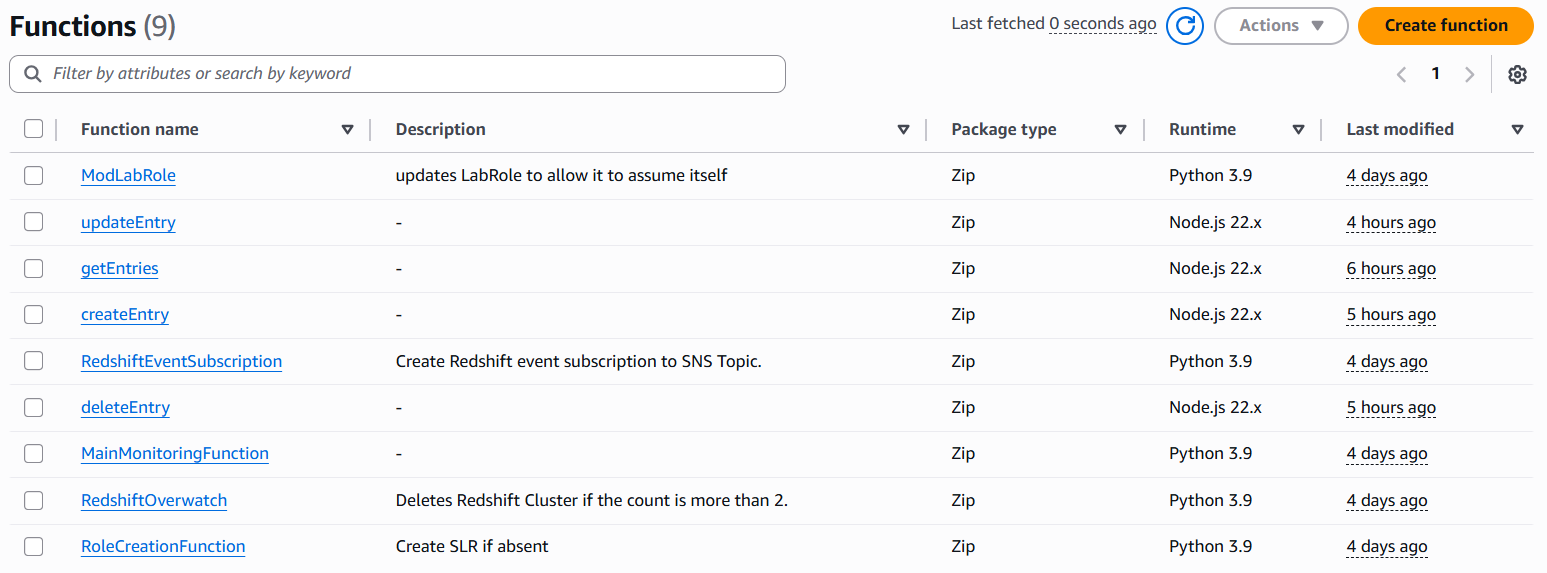
\includegraphics[scale=0.4]{lambda.png}
  \caption{Lambda в AWS Management Console}
\end{figure}

\medskip

\noindent\textbf{Стъпка 4.} Конфигуриране на API Gateway.\\
\noindent\textbf{4.1.} Създаване на Rest API. Избрана е REST архитектура, тъй като тя е стандартен и доказан подход за изграждане на уеб API-та. Тя е stateless (безсъстоятелна), което я прави изключително мащабируема и лесна за интегриране с клиентски приложения, като осигурява ясен и предвидим начин за взаимодействие с ресурсите на бекенда чрез стандартни HTTP методи.
\\
\\
API name: JournalAPI,\\
Region: us-east\\

 \begin{figure}[H]
\centering
    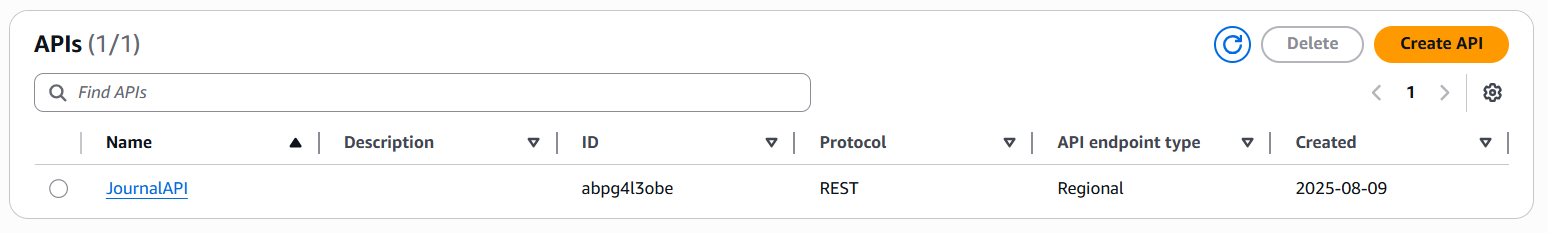
\includegraphics[scale=0.4]{api.png}
  \caption{APIs в AWS Management Console}
\end{figure}

\noindent\textbf{4.2.} Създаване на Authorizer. Авторизаторът е необходим, за да се осигури сигурност на API-то. Той интегрира API Gateway с Cognito User Pool, което позволява да се валидират потребителските токени (JWT) преди да се изпълни съответната Lambda функция. По този начин се гарантира, че само автентикирани потребители могат да достъпват и управляват своите дневникови записи, като се предотвратява нерегламентиран достъп.
\\
\\
Authorizer name: CognitoJournalAuthorizer
Authorizer ID: 2kwe3z

 \begin{figure}[H]
\centering
    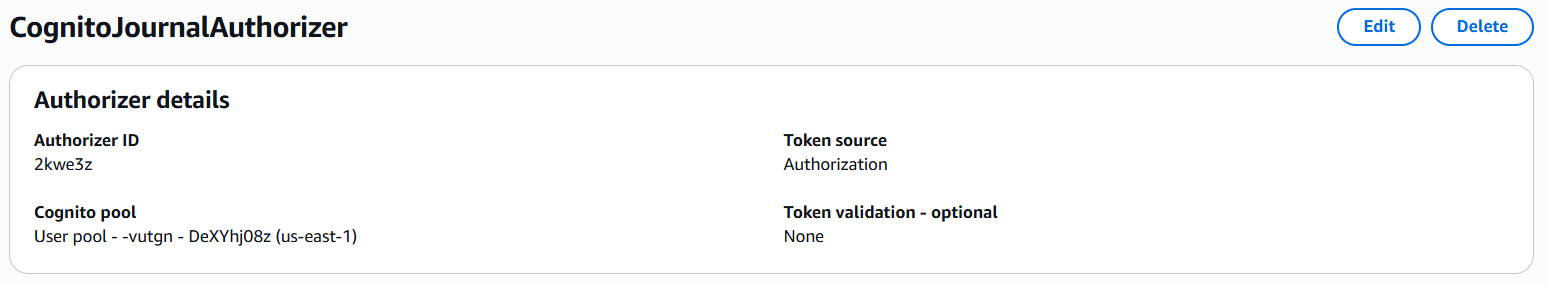
\includegraphics[scale=0.4]{authorizer.png}
  \caption{Authorizer в AWS Management Console}
\end{figure}

\noindent\textbf{4.3.} Създаване на ресурси и методи и свързване с lambda функциите. В API Gateway, ресурсите представляват пътищата (endpoints) на API-то, като например \texttt{/entries}. Методите са HTTP глаголите (GET, POST, PUT, DELETE), които се асоциират с тези ресурси. Всеки метод се интегрира с конкретна Lambda функция: \texttt{GET /entries} се свързва с \texttt{getEntries} Lambda функцията, \texttt{POST /entries} – с \texttt{createEntry}, \texttt{PUT /entries/\{entryId\}} – с \texttt{updateEntry}, \texttt{DELETE /entries/\{entryId\}} – с \texttt{deleteEntry}. Това позволява на клиентското приложение да изпраща заявки към специфични URL-и, които автоматично се пренасочват към правилната бекенд логика.

 \begin{figure}[H]
\centering
    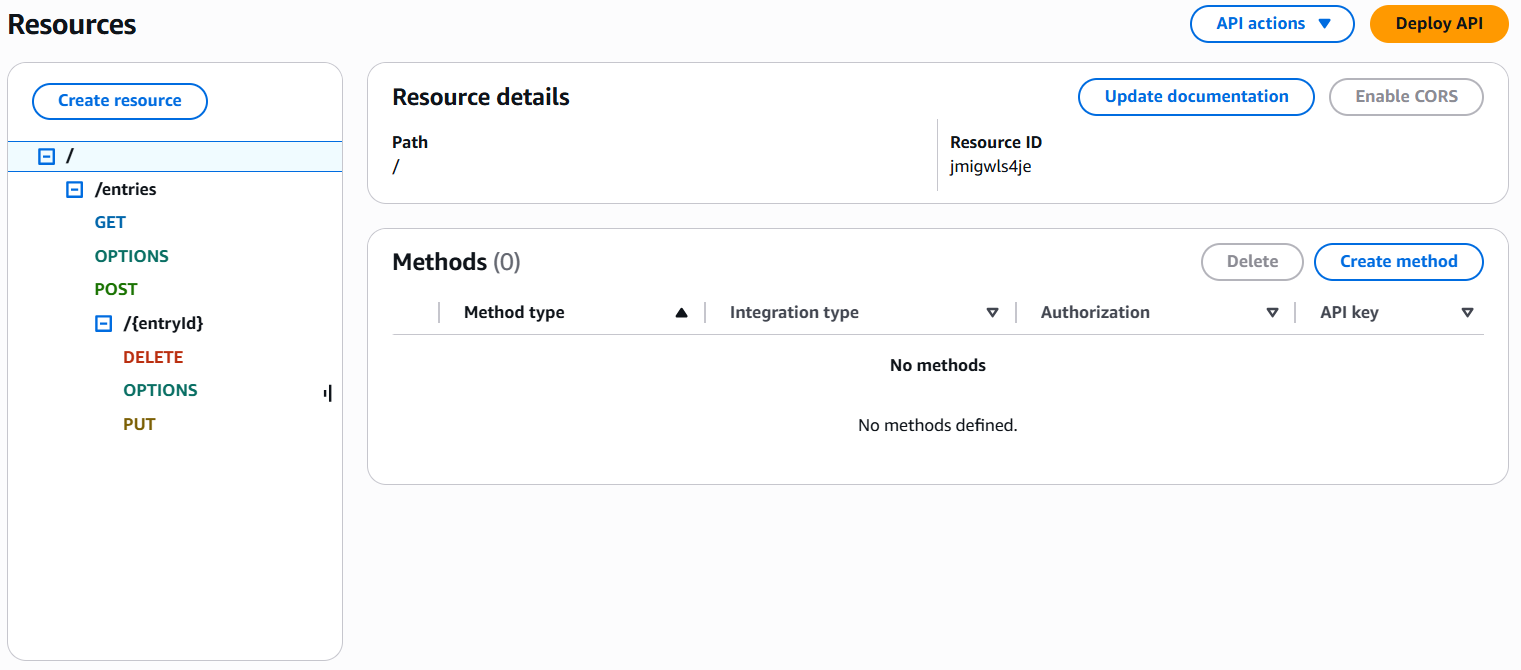
\includegraphics[scale=0.4]{api_resourses.png}
  \caption{JournalAPI Resourses в AWS Management Console}
\end{figure}

\noindent\textbf{4.4.} Активиране на CORS. Активирането на CORS (Cross-Origin Resource Sharing) е задължително, защото фронтенд приложението е хоствано на един домейн (S3 bucket), докато API Gateway се намира на друг. Без активиран CORS, уеб браузърите ще блокират заявките от фронтенда към бекенда поради своята политика за сигурност, известна като Same-Origin Policy.
\\

\noindent\textbf{4.5.} Deploy на API.\\
Stage Name: v1,\\
Invoke URL: https://abpg4l3obe.execute-api.us-east-1.amazonaws.com/v1.

 \begin{figure}[H]
\centering
    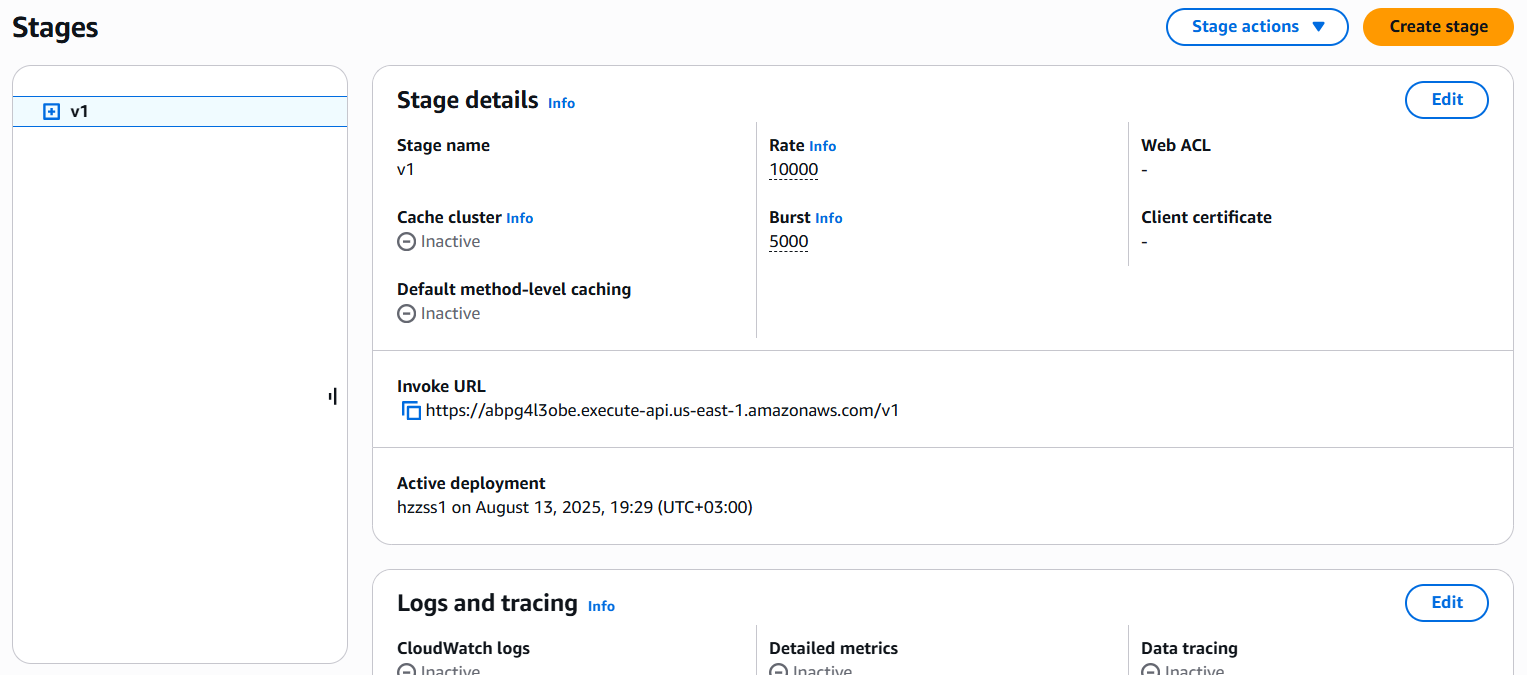
\includegraphics[scale=0.4]{stage.png}
  \caption{JournalAPI Stages в AWS Management Console}
\end{figure}

\medskip

\noindent\textbf{Стъпка 5.} Създаване на S3 Bucket за статичен уеб хостинг.\\
Bucket Name: journal-frontend-bucket-4620,\\
Bucket Website Endpoint: http://journal-frontend-bucket-4620.s3-website-us-east-1.amazonaws.com\\

 \begin{figure}[H]
\centering
    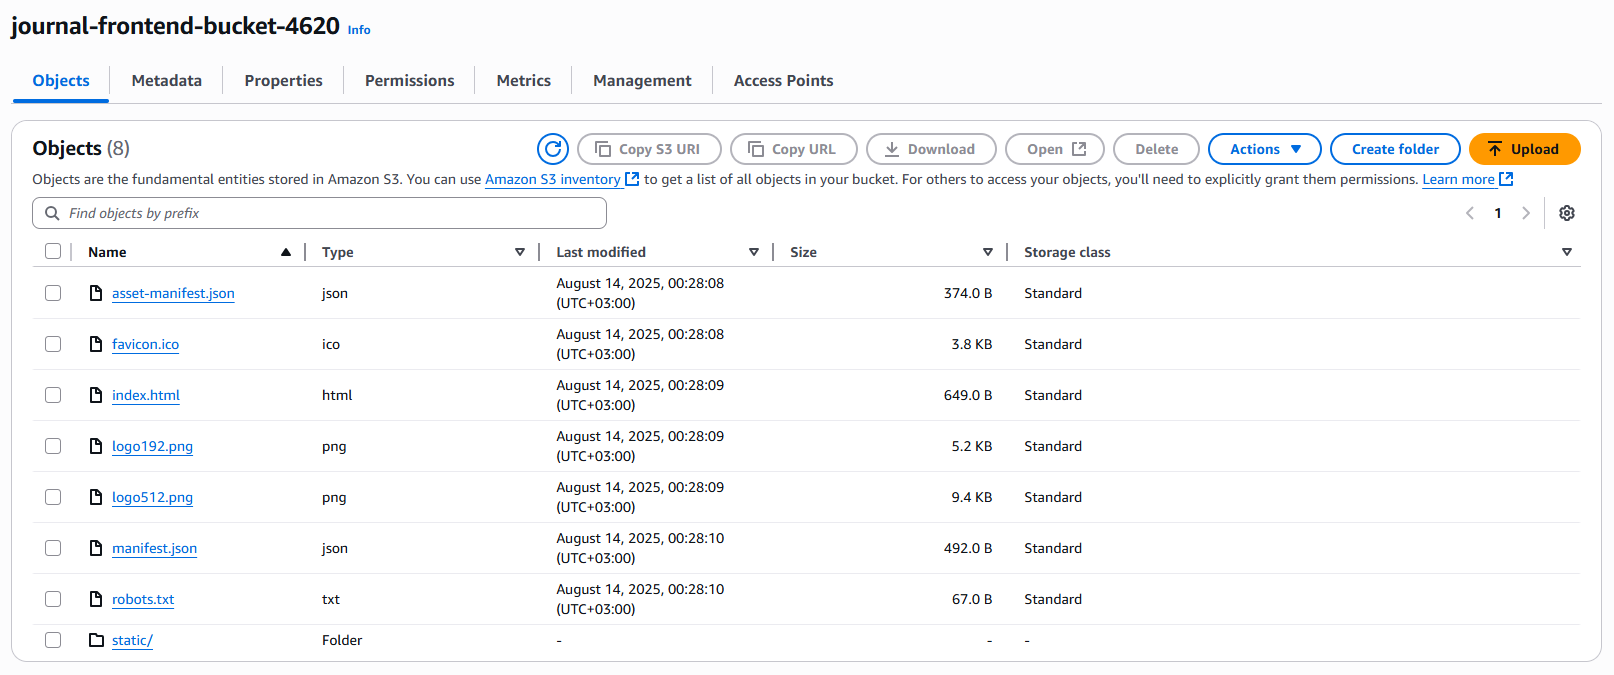
\includegraphics[scale=0.4]{s3.png}
  \caption{S3 Bucket в AWS Management Console}
\end{figure}

\medskip

\section{Кратко ръководство за потребителя}

\noindentТова ръководство ще ви запознае с интуитивния потребителски интерфейс на уеб дневника и как да използвате основните му функции. Приложението е разделено на няколко основни секции: автентикация, създаване на нов запис и преглед и управление на записи.

\medskip

\subsection{Регистрация и потвърждение на акаунт}
\begin{enumerate}
    \item Отворете уеб приложението в браузъра си. В горната част на екрана ще видите опции за "Sign in" и "Create account".
    \item Натиснете бутона \textbf{Create account}. Ще ви се отвори форма за регистрация.
    \item Въведете валиден имейл адрес и изберете парола. Натиснете бутона \textbf{Create account}.
    \item На посочения имейл адрес ще получите код за потвърждение (confirmation code). Въведете този код в полето \textbf{Confirmation code} и натиснете бутона \textbf{Confirm}.
    \item Вашият акаунт вече е регистриран и потвърден.
\end{enumerate}

 \begin{figure}[H]
\centering
    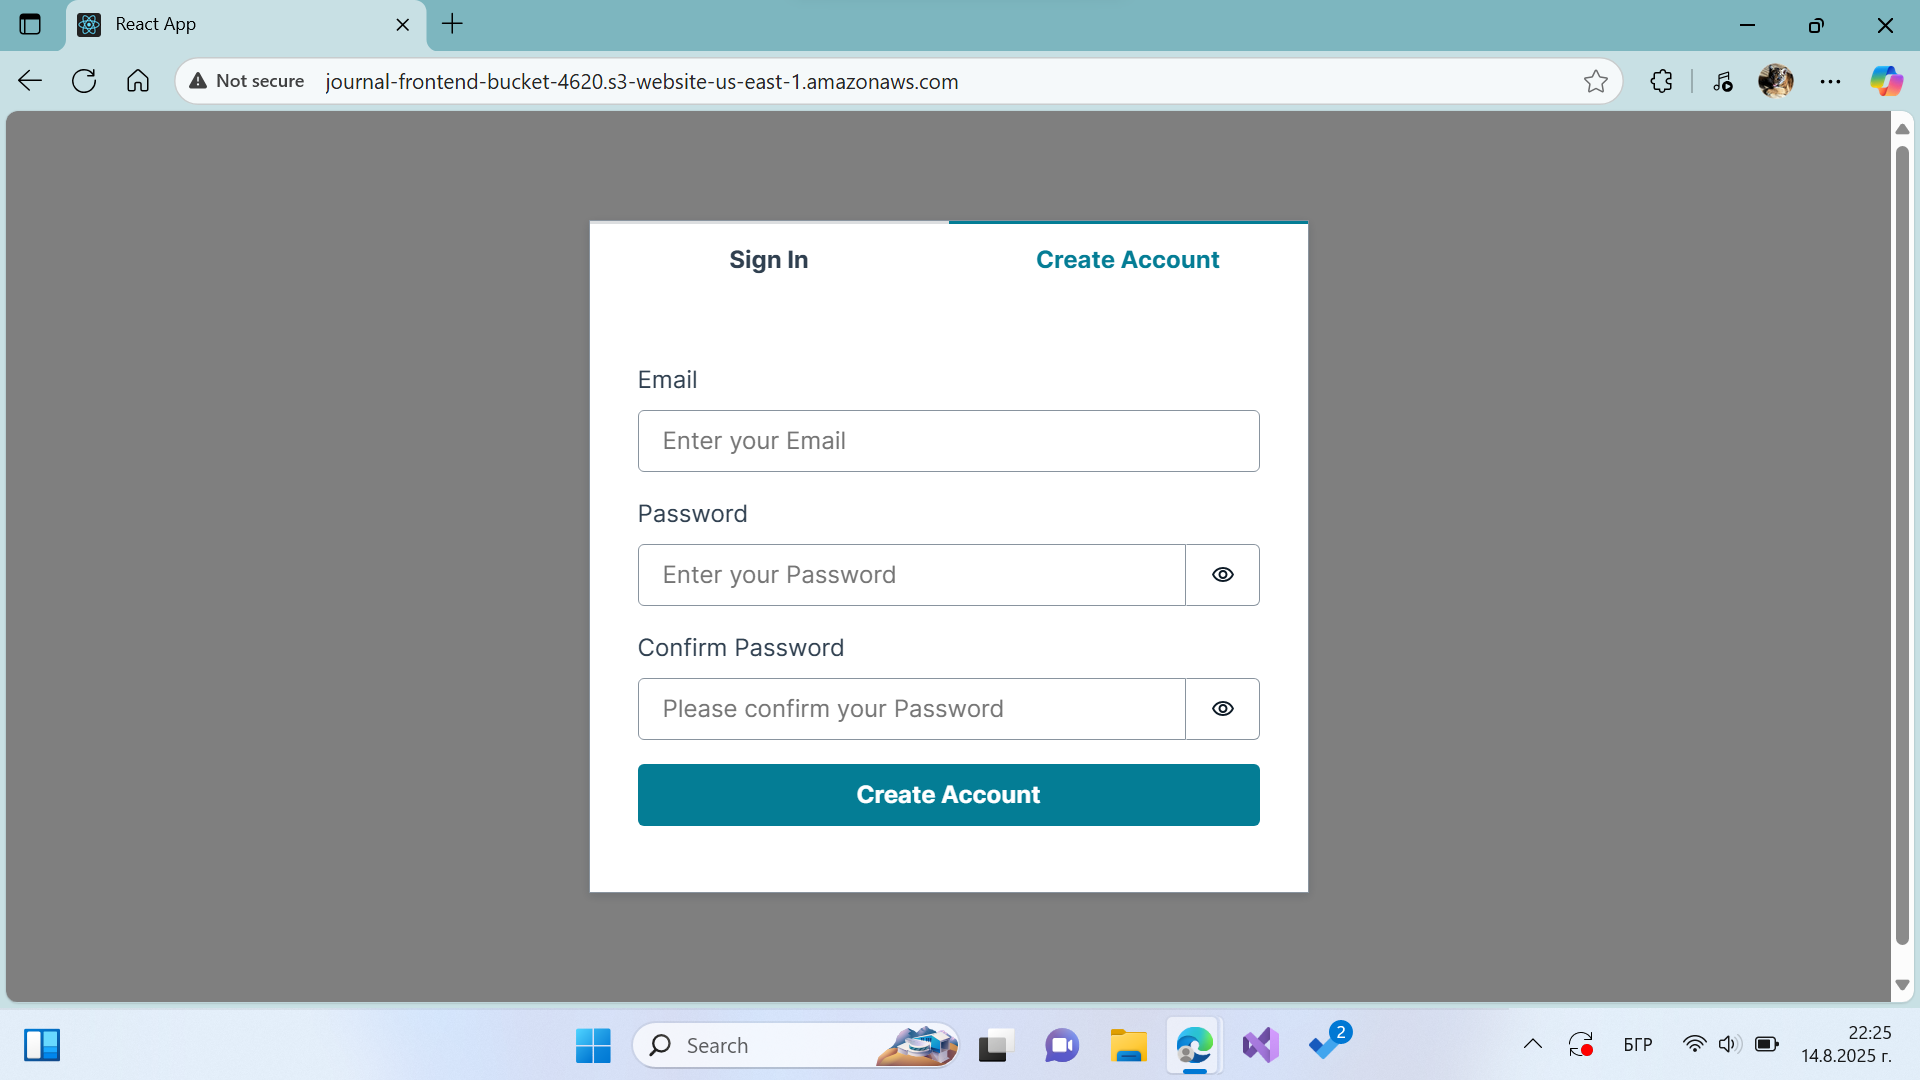
\includegraphics[scale=0.4]{create_account.png}
  \caption{Екран за създаване на акаунт}
\end{figure}

\subsection{Вход в системата}
\begin{enumerate}
    \item Отворете уеб приложението в браузъра си. 
    \item Въведете имейла и паролата, които сте използвали при регистрацията.
    \item Натиснете бутона \textbf{Sign in}. Ще бъдете пренасочени към главната страница на дневника.
\end{enumerate}

\begin{figure}[H]
    \centering
    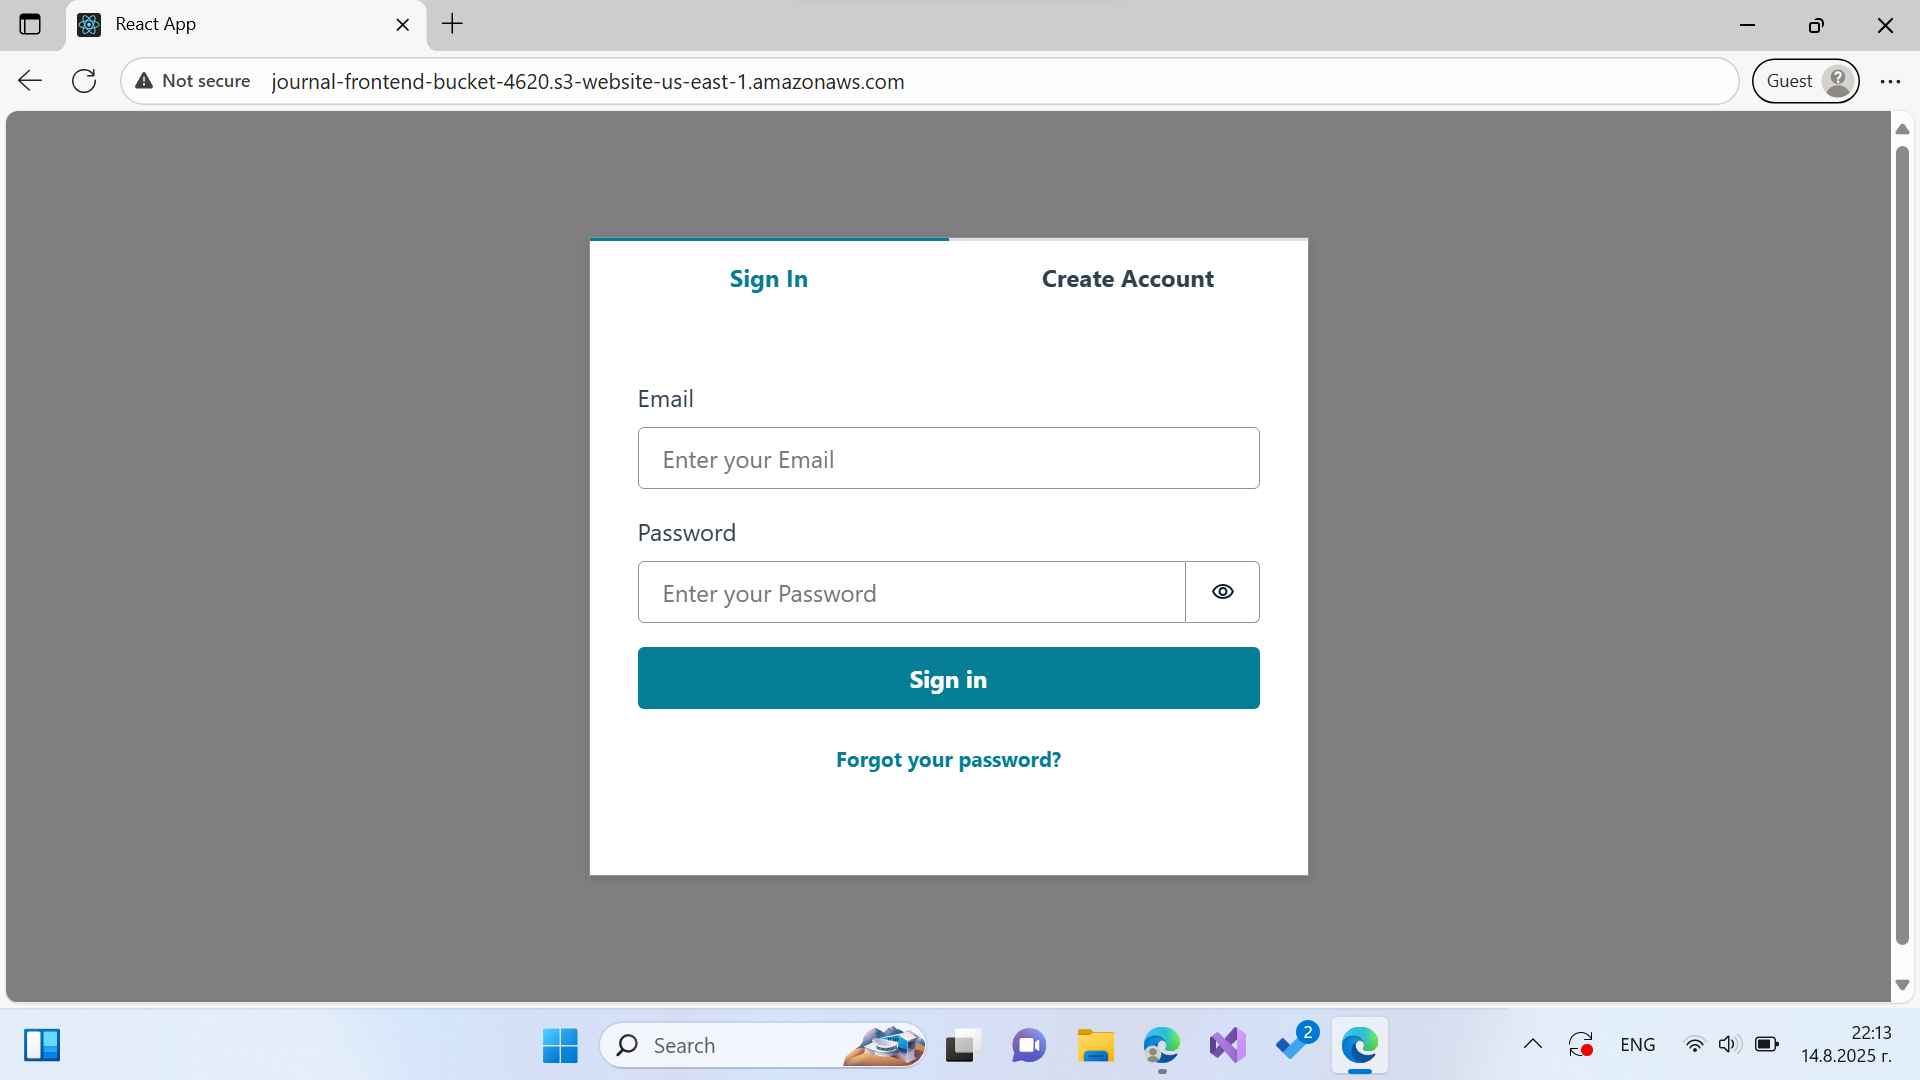
\includegraphics[scale=0.4]{sign_in.png}
    \caption{Екран за вход в системата}
\end{figure}

\subsection{Работа със записи в дневника}
Работата със записи в дневника се извършва през основната страница.

\begin{figure}[H]
    \centering
    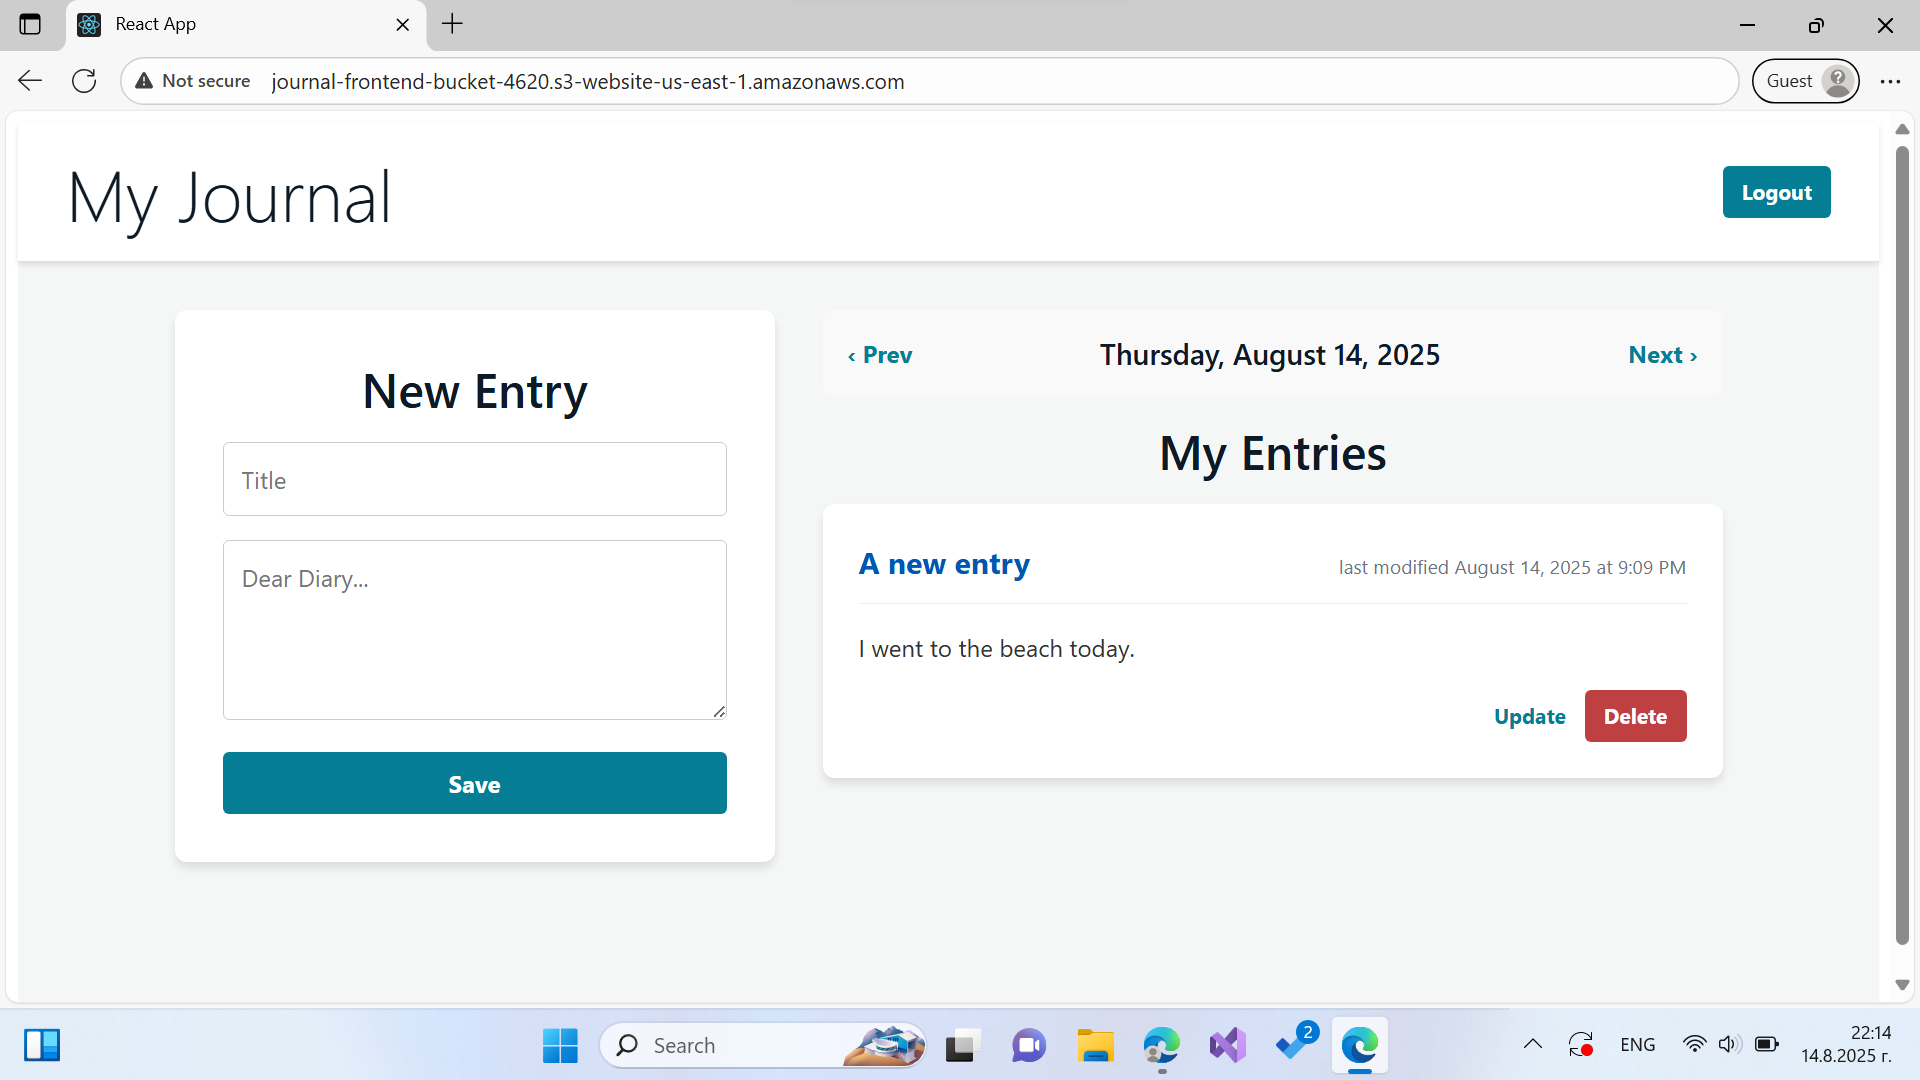
\includegraphics[scale=0.4]{main_page.png}
    \caption{Основен екран}
\end{figure}

\begin{enumerate}
    \item \textbf{Създаване на нов запис:}
    \begin{itemize}
        \item На главната страница ще видите секция \textbf{New Entry}.
        \item Въведете заглавие на записа в полето \textbf{Title}.
        \item Въведете съдържанието на записа в текстовото поле \textbf{Dear diary...}.
        \item Натиснете бутона \textbf{Save}. Новият запис ще се появи в секцията \textbf{My Entries}, сортиранa по дата на създаване на записите.
    \end{itemize}
    
    \item \textbf{Преглед на записи:}
    \begin{itemize}
        \item В секцията \textbf{My Entries} се показват всички ваши записи.
        \item Можете да навигирате между различните дати, като използвате бутоните \textbf{Prev} (предишен) и \textbf{Next} (следващ).
    \end{itemize}
    
    \item \textbf{Редактиране на запис:}
    \begin{itemize}
        \item До всеки запис в списъка има бутони за управление.
        \item Натиснете бутона \textbf{Update}, за да промените заглавието или съдържанието на съществуващ запис.
        \item След като направите промените, натиснете отново \textbf{Update}, за да ги запазите.
    \end{itemize}

    \item \textbf{Изтриване на запис:}
    \begin{itemize}
        \item За да изтриете запис, натиснете бутона \textbf{Delete} до съответния запис.
        \item Ще се появи изскачащ прозорец, който изисква потвърждение.
        \item Потвърдете, за да изтриете записа.
    \end{itemize}
\end{enumerate}

\subsection{Изход от системата}
За да прекратите сесията си, натиснете бутона \textbf{Logout}, който се намира в горния десен ъгъл на екрана.

\medskip

\section{Примерни данни}

При създаване на запис потребителят задава заглавие и съдържание. Входните данни и допълнителна информация за времето на създаване и редактиране се записват от бекенда в JournalEntries.

\begin{table}[H]
\centering
\caption{Примерни входни данни}
\begin{tabular}{ |l|l|l|l| }
 \hline
 \textbf{} & \textbf{Title} & \textbf{Content} & \textbf{Date} \\ \hline
 1 & A new entry & I went to the beach today. & 2025-08-14 \\ \hline
 2 & An old entry & I didn't go to the beach today. & 2025-08-13 \\ 
 \hline
\end{tabular}
\end{table}

\begin{table}[H]
    \caption{Примерно съдържание на JournalEntries}
    \centering
    \resizebox{\textwidth}{!}{%
    \begin{tabular}{|l|l|l|}
        \hline
        \textbf{} & \textbf{Запис 1} & \textbf{Запис 2} \\
        \hline
        \texttt{userId} & \texttt{34282458-2041-7085-9a84-29ae444e982f} & \texttt{34282458-2041-7085-9a84-29ae444e982f} \\
        \hline
        \texttt{entryId} & \texttt{3f0de891-f53d-4dd3-a797-62d9fb66b982} & \texttt{xqmf64j1-jjep-p2q1-uv78-pcq5dmporvyg} \\
        \hline
        \texttt{title} & \texttt{A new entry} & \texttt{An old entry} \\
        \hline
        \texttt{content} & \texttt{I went to the beach today.} & \texttt{I didn't go to the beach today.} \\
        \hline
        \texttt{createdAt} & \texttt{2025-08-14T18:09:17.631Z} & \texttt{2025-08-13T10:05:47.623Z} \\
        \hline
        \texttt{updatedAt} & \texttt{2025-08-14T18:09:17.631Z} & \texttt{2025-08-14T18:10:45.438Z} \\
        \hline
    \end{tabular}
    }
\end{table}

\medskip


\section{Описание на програмния код}

\noindent Програмният код е разделен на няколко модула, които отговарят за различни аспекти на сървърлес архитектурата. Всеки модул е реализиран като AWS Lambda функция, обработваща конкретни API заявки.

\subsection{Модул за автентикация (Cognito User Pool)}
Този модул отговаря за управлението на потребителските идентичности. Той осигурява сигурна регистрация и вход в системата. Кодът на този модул включва логика за:
\begin{itemize}
    \item Регистриране на нов потребител с имейл и парола.
    \item Изпращане на код за потвърждение по имейл.
    \item Потвърждаване на акаунт с получения код.
    \item Вход в системата и генериране на JWT (JSON Web Token) за автентикация.
\end{itemize}
Въпреки че самият код за тези операции е част от AWS Amplify или директно от SDK на AWS, логиката на приложението интегрира тези функционалности във фронтенд частта.

\subsection{Модул за управление на записи (AWS Lambda функции)}
Това е сърцето на бекенд логиката, реализирана чрез четири отделни Lambda функции. Всяка функция е проектирана да бъде отговорна само за една операция (single responsibility principle).

\begin{itemize}
    \item \texttt{createEntry.js}: Тази функция се извиква при POST заявка към \texttt{/entries}. Тя получава данни за заглавие и съдържание, генерира уникални идентификатори (\texttt{entryId}, \texttt{createdAt}, \texttt{updatedAt}) и съхранява новия запис в DynamoDB таблицата.
    \item \texttt{getEntries.js}: Изпълнява се при GET заявка към \texttt{/entries}. Тя прави заявка към DynamoDB, използвайки \texttt{userId} от автентикирания потребител, за да върне всички дневникови записи за деня, сортирани по час на създаване.
    \item \texttt{editEntry.js}: Отговаря на PUT заявки към \texttt{/entries/\{entryId\}}. Функцията получава новите данни за запис и ги актуализира в DynamoDB, като предварително проверява дали потребителят, който прави заявката, е собственик на записа.
    \item \texttt{deleteEntry.js}: Тази функция се активира при DELETE заявка към \texttt{/entries/\{entryId\}}. Тя изтрива съответния запис от DynamoDB след проверка на правата на достъп на потребителя.
\end{itemize}

\subsection{Модул на клиентската част (React приложение)}
Клиентската част е разработена като Single Page Application (SPA) с React. Кодът включва:
\begin{itemize}
    \item Компоненти за потребителския интерфейс (страница за вход, регистрация, основен екран на дневника).
    \item Бизнес логика за извикване на API ендпойнтите, обработка на отговорите и управление на състоянието на приложението.
    \item Интеграция с AWS Amplify, което улеснява взаимодействието с Cognito и API Gateway.
\end{itemize}
Цялото приложение е статично хоствано в S3 bucket.

\medskip


\section{Приноси на студента, ограничения и възможности за бъдещо развитие}

В процеса на разработка е реализирано напълно функционално приложение за водене на дневник, което позволява създаване, преглед, редакция и изтриване на записи. Интерфейсът е интуитивен, а структурата на кода позволява лесно надграждане с нови модули и подобрения. \\

Сред основните ограничения на текущата версия е невъзможността за създаване на записи за минали дати. В настоящата реализация потребителят може да създава записи само за текущия ден. \\

Като възможност за бъдещо развитие се предлага:
\begin{itemize}
    \item Добавяне на функционалност за създаване на записи за минали дни, което би позволило въвеждането на пропусната информация.
    \item Имплементиране на търсене по ключови думи и филтриране.
    \item Експорт и импорт на данни във формат PDF или CSV.
\end{itemize}

\medskip


\section{Какво научих}
Основният принос от изпълнението на проекта беше придобиването на практически умения за работа с облачната платформа AWS.  
Научих се да интегрирам и конфигурирам услуги като \textit{DynamoDB}, \textit{Lambda}, \textit{API Gateway}, \textit{Cognito} и \textit{S3}, за да изградя пълноценна бекенд инфраструктура.  
Паралелно с това развих умения за структуриране на софтуерен код, работа с \LaTeX{} за създаване на документация и прилагане на добри програмни практики.


\newpage
 

\section{Списък с фигури и таблици}

\listoftables

\listoffigures

\medskip


\section{Използвани източници}
\noindent\href{https://aws.amazon.com/s3/}{[1] Amazon S3 Documentation}\\
\noindent\href{https://aws.amazon.com/cognito/}{[2] Amazon Cognito Documentation}\\
\noindent\href{https://aws.amazon.com/api-gateway/}{[3] Amazon API Gateway Documentation}\\
\noindent\href{https://aws.amazon.com/lambda/}{[4] AWS Lambda Documentation}\\
\noindent\href{https://aws.amazon.com/dynamodb/}{[5] Amazon DynamoDB Documentation}

\biskip

\end{document}